\documentclass{standalone}
\usepackage{tikz}
\usetikzlibrary{arrows}
\usepackage{fontspec}
    \setmainfont{Charis SIL}
\begin{document}
% In the preamble:

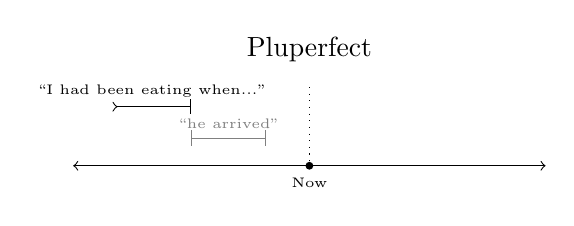
\begin{tikzpicture}[label distance=5mm]
    \draw [-, dotted] (0,1) node [] {} -- (-0,0) node[midway,above,sloped] (TextNode) {\tiny };
  \draw [<-, solid] (-3,0) node [] {} -- (-0.45,0) node[midway,above,sloped] (TextNode) {\tiny };
  \draw [-, solid] (-0.45,0) node [] {} -- (0.45,0) node[midway,above,sloped] (TextNode) {\tiny };
  \draw [->, solid] (0.45,0) node [] {} -- (3,0) node[midway,above,sloped] (TextNode) {\tiny };

  \draw [>-|, solid] (-2.5,0.75) node [] {} -- (-1.5,0.75) node[midway,above,sloped] (TextNode) {\tiny ``I had been eating when...''};
  \draw [gray, |-|, solid] (-1.5,0.35) node [] {} -- (-0.55,0.35) node[midway,above,sloped] (TextNode) {\tiny ``he arrived''};


      \draw (0,-0) node[circle,fill,inner sep=1pt]{};

 \draw (0,-0.4) node[anchor=south]{\tiny Now};

 \draw (0,1.2) node[anchor=south]{Pluperfect};

\end{tikzpicture}

\end{document}
